\documentclass[runningheads]{llncs}

\usepackage[T1]{fontenc}

\usepackage{graphicx} 

\usepackage{hyperref}
\usepackage{color}
\usepackage{booktabs}
\renewcommand\UrlFont{\color{blue}\rmfamily}

\raggedbottom

\begin{document}

\title{Monte Carlo Control and SARSA on TextFlappyBird: A Comparative Analysis}

\author{Jean-Vincent Martini}

\authorrunning{J.-V. Martini}

\institute{CentraleSupélec}
 
\maketitle   

\vspace*{-0.7cm}

\begin{abstract}
This report evaluates Monte Carlo Control and SARSA algorithms on state- and screen-based versions of the \href{https://gitlab-research.centralesupelec.fr/stergios.christodoulidis/text-flappy-bird-gym}{TextFlappyBird} environment. We analyze hyperparameter sensitivity, investigate policy transferability across configurations, and compare agent performance using rewards and scores. The report concludes with a discussion of observed trends and potential improvements.

\keywords{Reinforcement Learning \and Deep Learning \and Monte Carlo Control \and SARSA \and TextFlappyBird}
\end{abstract}
%
%
\vspace*{-0.7cm}

\section{Introduction and Problem Definition}

The objective of this project is to apply reinforcement learning (RL) techniques to master a simplified, terminal-based variant of the popular game Flappy Bird, known as Text Flappy Bird (TFB). In this environment, the player controls a simple unit-element character navigating through a series of pipe obstacles, aiming to maximize survival time and score. 

The problem is modeled using two distinct variations of the TFB environment, provided via a custom OpenAI Gym implementation: the simple version and the screen  version. Each version presents unique challenges in terms of observation space and complexity, requiring different approaches to policy learning and value estimation. To solve this environment, we formulate the gameplay as a Markov Decision Process and investigate two specific RL algorithms: the Monte Carlo Control method and the Sarsa($\lambda$) algorithm.

By implementing these agents, this report aims to evaluate and compare their convergence and overall performance across both environment versions. Furthermore, we conduct a sensitivity analysis on key hyperparameters and investigate the transferability of the learned policies to provide deeper insights into the behavior of both algorithms.

\section{Implementation Details}
\paragraph{Environment Setup and State Representation.} Both TFB variants share the
same dynamics: the action space consists of two actions, $0$ (Idle) and $1$ (Flap),
the agent receives a reward of $+1$ per step alive, and an episode terminates on
collision. They differ only in their observation space. The simple version provides
a tuple $(dx, dy)$ representing the horizontal and vertical distances to the center
of the nearest pipe gap, restricting the state space to the most critical navigational
information. The screen version instead exposes the full $20 \times 15$ game grid as
a \texttt{gym.spaces.Box}, where each cell encodes an entity: $0$ (background),
$1$ (alive player), $2$ (pipe), or $3$ (dead player), requiring the agent to
implicitly extract geometric features from the raw spatial layout.

\paragraph{Agents and Algorithms.} We implemented two classical RL algorithms. Both utilize an $\epsilon$-greedy exploration strategy with exponential decay. For the screen environment, two complementary state representations are used. In the hash-based variant, the raw grid array is serialized into a nested tuple usable as a dictionary key, preserving full grid information at the cost of a large, non-generalizing state space. In the tile-coding variant, a compact feature vector $(d_x, d_y)$ is extracted from the screen and encoded using $8$ overlapping tilings over a $4\times4$ grid, enabling generalization across nearby states through linear function approximation.

The Monte Carlo Control agent learns from complete episodes. At the end of each episode, the cumulative discounted return $G_t$ is computed backwards from the terminal state. The Q-values are updated for every visited state-action pair using a constant step-size $\alpha$:
$Q(S_t, A_t) \leftarrow Q(S_t, A_t) + \alpha (G_t - Q(S_t, A_t))$. 

The Sarsa($\lambda$) agent, in contrast, utilizes eligibility traces to propagate delayed rewards back to recently visited states more efficiently\cite{sutton2018reinforcement}. Our implementation increments an accumulating trace $E(s,a)$ upon visitation. The error $\delta_t$ and subsequent Q-value updates for all active traces are defined as:
$\delta_t = R_{t+1} + \gamma Q(S_{t+1}, A_{t+1}) - Q(S_t, A_t)$ and
$Q(s, a) \leftarrow Q(s, a) + \alpha \delta_t E(s, a)$.
To optimize memory and computational performance during training, any traces that decay below a negligible threshold ($1 \times 10^{-10}$) are dynamically deleted.


\section{Evaluation and Results}
\paragraph{Performance Comparison between Monte Carlo Control and SARSA.} Each agent
was trained for 25\,000 episodes and evaluated over 200 episodes (fewer for tile-coding
variants due to longer inference times) on the training configuration (\texttt{height=15},
\texttt{width=20}, \texttt{pipe\_gap=4}), with a step cap of 50\,000 per episode
(maximum score: 4999). Figure~\ref{fig:train_scores} shows the training curves and
Table~\ref{tab:results} summarizes evaluation results. Because the score distribution
is heavily skewed, the median is a more robust indicator of typical performance than
the mean, which is disproportionately influenced by rare high-scoring runs and often
comparable in magnitude to the standard deviation.

In the simple environment, both agents learned effective policies, though MCC proved
more stable at evaluation time, consistently achieving the maximum score of 4999, while
Sarsa's performance remained more unstable despite competitive training scores. In the
screen environment, tile coding was critical: both MCC and Sarsa with tile coding
achieved near-optimal performance at evaluation, whereas the hash-based agents
struggled to generalize across the large state space, yielding significantly lower
scores. The difference in performance between the two algorithms can be attributed to Sarsa's bootstrapping mechanism. The Q-value updates rely on the current estimate of the next state, which introduces variance during training, whereas Monte Carlo Control updates from complete episode returns, providing lower-variance estimates that prove more reliable in this setting.



\paragraph{Hyperparameter Sensitivity Analysis.} TODO

\paragraph{Transferability of Learned Policies through Different Environment Configurations.} TODO

\paragraph{Key Limitations When Applied to the Real Flappy Bird Game.} While some agents performed well in TFB, directly applying them to the original \href{https://github.com/Talendar/flappy-bird-gym}{Flappy Bird Gym} would face fundamental limitations. The simple-environment agents rely on a compact $(dx, dy)$  observation not natively provided by the original game, requiring an additional feature-extraction layer. The hash-based screen agents are even less transferable, as any change in resolution or layout produces entirely unseen states, rendering the learned Q-table useless. The tile-coding agents are the most promising candidates, since they also operate on extracted $(dx, dy)$ features and are robust to minor variations in the input space. However, they would still require careful tuning of the tile parameters and may struggle with the increased complexity and noise of the original game environment, which includes more intricate graphics, faster dynamics, and additional sources of variability not present in TFB. More broadly, all variants rely on tabular or linear representations that scale poorly to the visual complexity of the original game.

\section{Conclusion and Perspectives}

\clearpage
\appendix

\section{Figures}

\begin{figure}[ht]
    \centering
    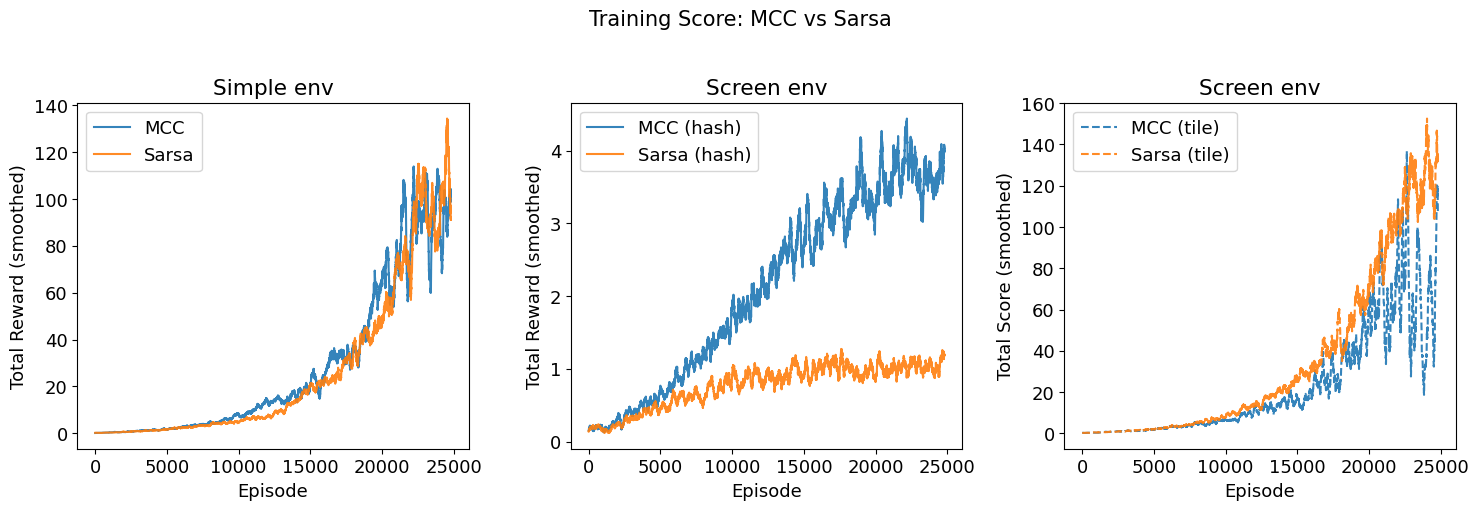
\includegraphics[width=0.8\textwidth]{figures/train_scores.png}
    \caption{Training scores for all agents and environment configurations. The curves are smoothed using a moving average with a window size of 100 episodes for better visualization.}
    \label{fig:train_scores}
\end{figure}

\begin{table}[ht]
\centering
\small
\resizebox{\textwidth}{!}{
\begin{tabular}{llrrrrrr}
\hline
\textbf{Agent} & \textbf{Env} & \textbf{Mean Rew.} & \textbf{Std Rew.} & \textbf{Mean Score} & \textbf{Std Score} & \textbf{Med.\ Rew.} & \textbf{Med.\ Score} \\
\hline
MCC        & v0        & 50000.0 &    0.0 & 4999.00 &   0.00 & 50000.0 & 4999.00 \\
Sarsa      & v0        &  7489.6 & 8028.2 &  747.66 & 802.82 &  4338.0 &  432.50 \\
MCC        & screen-v0 &    53.5 &   36.8 &    4.11 &   3.67 &    43.0 &    3.00 \\
Sarsa      & screen-v0 &    22.9 &   14.5 &    1.06 &   1.47 &    19.0 &    1.00 \\
MCC Tile   & screen-v0 & 50000.0 &    0.0 & 4999.00 &   0.00 & 50000.0 & 4999.00 \\
Sarsa Tile & screen-v0 & 50000.0 &    0.0 & 4999.00 &   0.00 & 50000.0 & 4999.00 \\
\hline
\end{tabular}}
\caption{Evaluation results per agent and environment configuration. The maximum possible reward is 50\,000 (corresponding to a score of 4999) due to the step cap.}
\label{tab:results}
\end{table}
\section{Figures for Hyperparameter Sensitivity Analysis}
% ---- Bibliography ----

\bibliographystyle{splncs04}
\bibliography{mybibliography}


\end{document}
